\section{商取引ゲーム}
 また,この「商取引システム」において,商取引で不正行為を防止できるインセンティブ設計を行うことができるのかを検証するするために,
  このシステムを商取引の仲介として用いる「商取引ゲーム」を次のように定義する.なお,ここでのゲームの$players$(システムの参加者達)は合理的に(期待利得の最も高い)戦略を決定するものとする.
  
  \subsection{ゲームの進め方}
   本稿での商取引は,以下の4つのステップで$seller$と$buyer$が交互に行動を展開するものとする.
  
    \begin{description}
      \item[step1] $seller$は商品$goods$とその価格を告知する
      \item[step2]  その商品の購入を希望する$buyer$が「商取引システム」に商取引の合意を報告する.
      \item[step3]  $seller$は「正当な行為」と「不正な行為」のどちらかの行動選択をする.ここで「正当な行為」を行った場合,$buyer$は契約通りの$goods$を受け取れ, 「不正な行為」を行った場合,$buyer$は契約通りの$goods$を受け取れないものとする.
      \item[step4]  $buyer$は商取引の「成功」か「失敗」かを「商取引システム」に報告する.この報告に基づき,「商取引システム」は$ seller$と$ buyer$の保有する通貨の量を調整する.
    \end{description}

  \subsection{ゲーム木}
    \begin{figure*}[h]
      \centering
      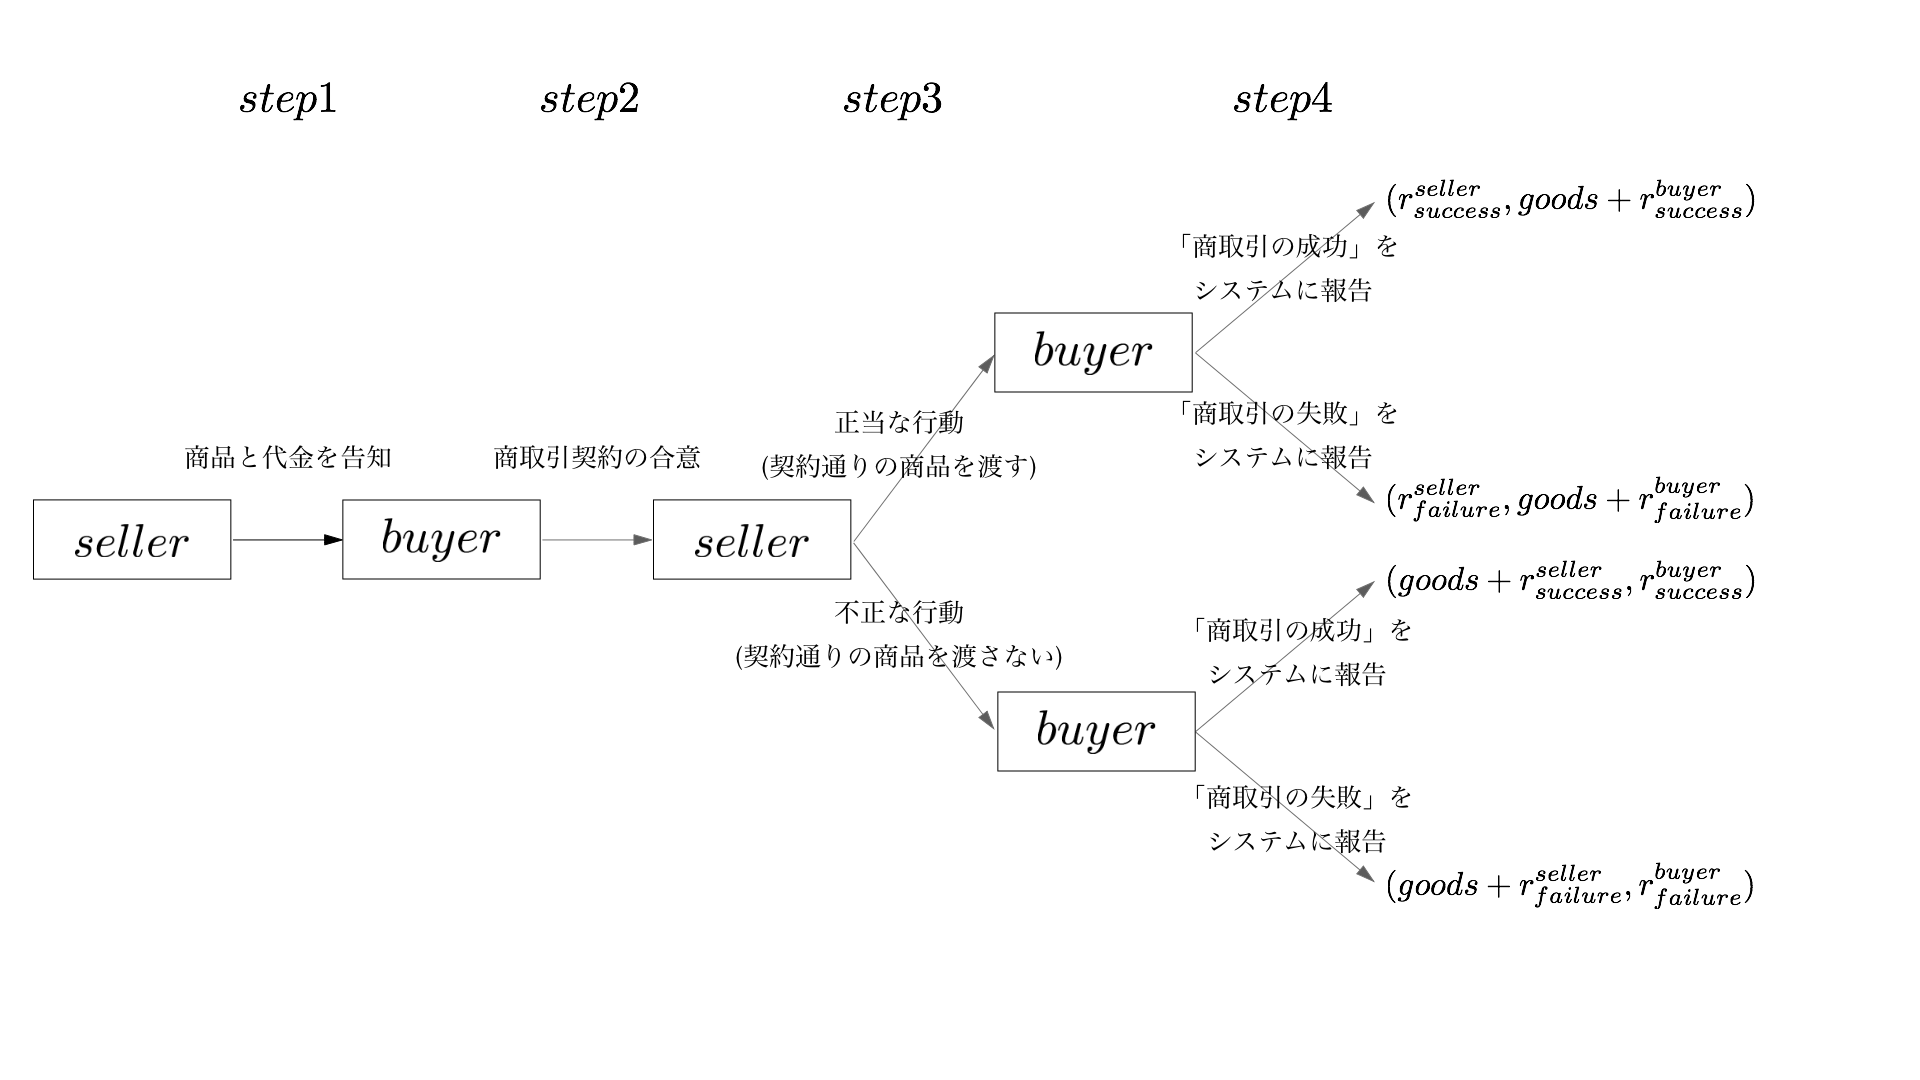
\includegraphics[width=1\linewidth]{./05_commerce-game/gametree.png}
      \caption{「商取引ゲーム」のゲーム木}
      \label{gametree}
    \end{figure*}
     先の商取引ゲームをゲームの木を用いて表すと図\ref{gametree}のようになる.\textbf{step1}と\textbf{step2}の時点では商取引の結果が変化することはなく,\textbf{step3}で$seller$が「正当な行為」をとるか否かと,\textbf{step4}での$buyer$からの報告によってのみ商取引の結果は変化する.また,「商取引システム」からは「行動観察不可の条件」より$seller$と$buyer$がどの行動をとったかはわからないため,\textbf{step4}での$buyer$の報告にのみ基づいて$seller$と$buyer$の保有する通貨の量を調整しなければならない.つまりは商取引の結果①と③,②と④はそれぞれ$goods$を除く利得は同じでなくてはならない.
  
  \subsection{非協力戦略型ゲーム}
    \newcommand{\successseller}{
      \begin{tabular}{c}
        $(r^{seller}_{success},$\\
        $goods+r^{buyer}_{success})$
      \end{tabular}
    }
    \newcommand{\successbuyer}{
      \begin{tabular}{c}
        $(goods+r^{seller}_{success},$\\
        $r^{buyer}_{success})$
      \end{tabular}
    }
    \newcommand{\fseller}{
      \begin{tabular}{c}
        $(r^{seller}_{failure},$\\
        $goods+r^{buyer}_{failure})$
      \end{tabular}
    }
    \newcommand{\fbuyer}{
      \begin{tabular}{c}
        $(goods+r^{seller}_{failure},$\\
        $r^{buyer}_{failure})$
      \end{tabular}
    }

    \begin{table*}[h]
      \begin{tabular}{|l|l|l|l|l|l|}
      \hline
      \multicolumn{2}{|l|}{\multirow{2}{*}{}} & \multicolumn{4}{l|}{$buyer$} \\ \cline{3-6}
      \multicolumn{2}{|l|}{}                  &$s^{buyer}_1$&$s^{buyer}_2$&$s^{buyer}_3$&$s^{buyer}_4$\\ \hline
      \multirow{2}{*}{$seller$}
      &$s^{seller}_1$&\successseller&\successseller&\fseller&\fseller\\ \cline{2-6}
      &$s^{seller}_2$&\fbuyer&\successbuyer&\fbuyer&\successbuyer\\ \hline
      \end{tabular}
      \caption{非協力戦略型ゲームとして表した「商取引ゲーム」の利得表}
      \label{gametable}
    \end{table*}
      
      また,この商取引のモデルは,第3ステップ以降の$seller$の行動選択と,それに対する第4ステップの$ buyer$の行動選択を,非協力戦略型ゲームとしてとらえられる.ここで,戦略$ s^{player}_{n}$を$ player$(ここでは$seller$か$buyer$)の取りうる戦略番号$n$の戦略として,$ seller$と$ buyer$のそれぞれの戦略は以下のように定義する.\\
      
      \begin{description}
        \item[$s^{seller}_1$]… 正当な行為を行う
        \item[$s^{seller}_2$]… 不正な行為を行う
        \item[$s^{buyer}_1$]… $ seller$が正当な行為をとった場合は「成功」を,不正な行動をとった場合は「失敗」を報告する
        \item[$s^{buyer}_2$]… $ seller$が正当な行為をとった場合は「成功」を,不正な行動をとった場合は「成功」を報告する
        \item[$s^{buyer}_3$]… $ seller$が正当な行為をとった場合は「失敗」を,不正な行動をとった場合は「失敗」を報告する
        \item[$s^{buyer}_4$]… $ seller$が正当な行為をとった場合は「失敗」を,不正な行動をとった場合は「成功」を報告する
      \end{description}
      
      また,商取引終了時の$ player$の保有する通貨量の変化によって生じる利得を,第4ステップでの報告が「成功」だった場合は$ r^{player}_{success}$,「失敗」だった場合は$ r^{player}_{failure}$とし,商品の所有によって生じる利得を$ goods$と表す.
      ここで,$ seller$と$ buyer$の任意の戦略組$ (s^{seller}_n, s^{buyer}_n)$の際の$ seller$と$ buyer$の各利得は表\ref{gametable}のようになる.
      